\subsubsection{Minuta de reunião (26-Agosto-2015)}

\begin{tabbing}
  Local \= xxx \kill
  Local \> : LEAD \\
  Data  \> : 26 de Agosto de 2015 \\
  Hora  \> : 13:00
\end{tabbing}

%---------------------------------------------------------------------
\participantes{
  \gabriel,
  \julia,
  \estevão,
  \elael,
  \renan,
  \ramon.

}

\textbf{Aprovação da minuta}

\textbf{Update semanal do Projeto EMMA}
   							
\textbf{\alana.} 
	\begin{itemize}
		\item \textbf{Tarefas concluídas:}
			\begin{itemize}    
				\item Prestação de contas.
			\end{itemize}
		
		\item \textbf{Novas tarefas:}
			\begin{itemize} 
				\item Relatório de Auditoria.
				\item Ofícios.
			\end{itemize}
	\end{itemize}   		
						
\textbf{\gabriel.} 
	\begin{itemize}
			\item Resumiuem uma planilha suas reuniões com fornecedores de sensores,
			comparando preços, capacidades e aplicações para o projeto.
			\item Implementação de driver ROS para ROCK do laser scan em progresso.
			\end{itemize}
		
		\item \textbf{Novas tarefas:}
			\begin{itemize} 
				\item Incluir novas cotações para sensores Velodine e Leica.
				\item Continuar implementação do driver do Laser Scan.
				\item Estudar possibilidades para alinhamento de nuvem de pontos.
			\end{itemize}

					
			
   \textbf{\estevão.} 
	\begin{itemize}
		\item \textbf{Tarefas concluídas:}
			\begin{itemize}    
				\item Apresentou com Renan dados para solução da escotilha inferior sem
				graus de liberdade.
				\item Conseguiu dois orçamentos maquete.
				
			\end{itemize}
		
		\item \textbf{Novas tarefas:}
			\begin{itemize} 
			    \item Conceito sobre solução de cabeamento.
			    \item Finalizar o processo de serviço para maquete: pagamento, e
			    justificativa técnica caso não haja 3 ofertas disponíveis no mercado.
			    \item Estágiário: delegar novas tarefas de acordo com sua necessidade.
			\end{itemize}
	\end{itemize}

	  \textbf{\renan.} 
	\begin{itemize}
		\item \textbf{Tarefas concluídas:}
			\begin{itemize}    
				\item Fez um estudo da dos tolerância no end effector. 
			\end{itemize}
		
		\item \textbf{Novas tarefas:}
			\begin{itemize} 
			    \item Frame por frame para ver hardcoating para cada ângulo da pá.
			    \item Verificar com staff ESBR e Rijeza sobre estrutura da unidade
			    geradora de Itaipú e Santo Antônio.
			    \item Comunicar a Rijeza os pontos fracos e fortes de ambas soluções.
			\end{itemize}
	\end{itemize}	
	
	
	  \textbf{\elael.} 
	\begin{itemize}
		\item \textbf{Tarefas concluídas:}
			\begin{itemize}    
				\item Relatório CITENEL.
				\item Cotações para Point Laser. 
			\end{itemize}
		
		\item \textbf{Novas tarefas:}
			\begin{itemize} 
			    \item Explorar PCL através de amostra online.
			    \item Alinhar dus nuvem de pontos.
			    \item Adicionar cotações point laser (Laser Pontual utlizado para medir
			    distâncias entre objetos).
			\end{itemize}
	\end{itemize}			
			
			
   \textbf{\julia.} 
	\begin{itemize}
		\item \textbf{Tarefas concluídas:}
			\begin{itemize}    
				\item Apresentação da estrutura de projeto para EMMA, fases relacionadas
				criação e desenvolviemnto da interface gráfica do robô.
			\end{itemize}
		
		\item \textbf{Novas tarefas:}
			\begin{itemize} 
			    \item Apresentação de Fase de ´Descoberta´ para o time, como se
			    estrutura a pesquisa e de que formas ela alimenta os entregáveis do
			   para a elaboração da interface do usuário. 
			    \item Documentação e coordenação de tarefas da semana.
			\end{itemize}
	\end{itemize}		



\textbf{Agenda para a próxima reunião:}
  \begin{itemize}
    \item Resultado de pesquisas individuais.
    \item Novas tarefas \& recomendações.
  \end{itemize}


\vspace{5mm}%
\parbox[t]{70mm}{
  Aprovado por: \\[5mm]
  \centering
  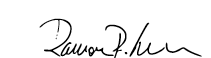
\includegraphics[width=65mm]{figs/logo/assinatura-ramon.png} \\[-4mm]
  \rule[2mm]{70mm}{0.1mm} \\
  \ramon \\[1mm]
  Coordenador do Projeto \\
}

%---------------------------------------------------------------------
\fim